\documentclass[conference]{IEEEtran}
\usepackage{textcomp}
\usepackage{lscape}
\usepackage{graphicx}
\usepackage{cite}
\usepackage{amsmath}
\usepackage{gensymb}
\usepackage[T1]{fontenc}
\usepackage[hyphens]{url}
\usepackage{hyperref}
\usepackage{ragged2e}
\setlength{\textfloatsep}{3pt}
\setlength{\floatsep}{3pt}
\setlength{\parindent}{0pt}
\usepackage[bottom=1.5cm, top=1.5cm, left=1.5cm, right=1.5cm]{geometry}
\begin{document}
\bstctlcite{IEEEexample:BSTcontrol}
\twocolumn[
\centering
\huge{ELEN4002: Digital Estimation of Body Mass Index}
\vspace{6pt}
\linebreak
\large{Darrion Singh (1056673)}
\justify
\small{\textbf{Abstract:} The following reports the design and implementation of an application used to estimate Body Mass Index from a photograph.
The total duration of the project was six weeks.
The application consisted of a feature extraction layer and a machine learning layer.
The dataset collected to train the machine learning layer consisted of 465 anonymised people's photographs.
The program detected a reference object of known dimensions located in each photograph, and subsequently estimated the dimensions of the person in the photograph.
Dimensions were chosen at the location of common body fat deposits, and along with person's estimated silhouette area and estimated height, were used to train three Multilayer Perceptron (MLP) models that estimated BMI -- one for the front photograph, another for the side photograph, and finally, one that compensated for errors between the front and side estimations, and was the final output of the program.
The results of the final model BMI estimation showed a mean estimation accuracy ranging between 79\% and 92\% for the various categories of BMI, namely Underweight (< 18.5), Healthy (18.5 -- 25), Overweight (25 -- 30), or Obese (> 30).
Furthermore, the spread of error showed that about 61\% of participants had an error less than 10\%, and about 89\% of participants had an error less than 25\%.
Predictions on the total dataset had a mean absolute error of 3.2, and standard deviation of 3.9.}
\vspace{6pt}
]

\section{Introduction}
The Body Mass Index (BMI) is a screening tool used to indicate whether one's body mass is healthy for their corresponding height \cite{nhsBMI}.
Whilst not an accurate diagnostic tool, the BMI provides a healthy body mass range for a particular height as it takes natural body shape variations into account \cite{nhsBMI}.
Unfortunately, the distance between rural areas and clinics prevent inhabitants of that area from regular medical checkups, where a medical practitioner might require to measure and track ones height and mass.
A solution to both the above mentioned problems would be the creation of a tool that would provide a medical practitioner with this information without the need for the patient to be physically present.
The following report presents the design and implementation of program that estimates BMI from a front and side photograph using a mixture of Computer Vision and Machine Learning.
The School of Electrical and Information Engineering (EIE) have collaborated with the Peri-Natal HIV Research Unit (PHRU) for this project.

\section{Background}
The Assumptions, Constraints, and Success Criteria have been re-evaluated and refined from that which was described in the Project Plan in Appendix 3.
Note that the Optional Criteria for this project (Section IID of Appendix 3) remain unchanged.
\subsection{Project Concept} \label{concept}
The aim of this project is to estimate the BMI of a person by creating a program which accepts a front and side photograph of that person.
The program will extract body shape data from the photographs with the use of Computer Vision, and estimate their BMI based on their body shape data using Machine Learning.

The purpose of such a tool has vast applications in the medical field, whether it be used as a time-efficient means of tracking the progress of a disease/disorder that affects ones mass, or for a simple indication of ones own health.
Furthermore, a possible extension of this tool would be using it to classify which category of BMI one falls into: Underweight (< 18.5), Healthy (18.5 -- 25), Overweight (25 -- 30), or Obese (> 30).

\subsection{Assumptions \& Constraints}
\begin{itemize}
	\item As to provide the least chance of a false human body outline being detected, we assume that any person being photographed is staged in front of a uniform background, such as a wall whose colour significantly contrasts with that of the patient and their clothes.
	All photographs used to train the machine learning algorithm should abide by the same assumption.
	\item In order to provide a measurement reference, the person in each photograph should be standing next to a reference object (RO) of known dimensions, such as a piece of standard A4 paper. The colour and dimensions of the piece of paper should be the same throughout the training dataset.
	\item This RO is present in the photographs during testing or usage of the application.
	\item All subjects in the photographs stand alongside and in line with the RO, i.e. if the RO is stuck to a wall, the subject is standing against the wall.
	\item The distance between the camera and the subjects being photographed is constant and far enough away to capture the subject's full body photograph.
	\item Subjects have a maximum height of two meters.
	\item The time frame for this project is six weeks, with a total budget of R1200.
\end{itemize}

\subsection{Success Criteria}
\begin{itemize}
	\item The program should provide an average accuracy of 75\% for it to be classified as a potential viable solution.
	\item To be considered a working prototype, it should provide an average accuracy of 85\%.
	\item To be considered a completed product, it should provide a minimum average accuracy of 95\% across all age, gender, and mass groups.
	\item BMI estimation can occur with photographs of clothed people.
	\item The final solution is a robust desktop application that can be easily used by a medical practitioner.
	\item The solution should be camera resolution-independent.
\end{itemize}

\section{Literature Review}
The following literature were those most relevant to the estimation of BMI or relevant to the design choices made.
Further literature was consulted, the findings of which can be seen in the "Literature Review" section of Appendix 3.
\subsection{Weight and Diameter Estimation of Apples}
Comert et al. aims to estimate the mass of an apple through image processing and machine learning techniques \cite{comert}.
The process involves performing edge detection on the original image using the Prewitt edge extraction algorithm, which creates a binary image containing the edges in the original image.
The binary image then undergoes Closing, filtering and Opening.

Closing is the process of performing Dilation followed by Erosion on an image, whilst Opening is the process of performing Erosion followed by Dilation on an image \cite{opening,closing}.
Dilation is a morphological operation whereby the value (intensity) of a pixel is increased to that of the pixel in its neighbourhood with the highest intensity \cite{mathworksdilationerosion}.
Erosion is a morphological operation whereby the value of a pixel is decreased to that of the pixel in its neighbourhood with the lowest intensity \cite{mathworksdilationerosion}.

This is done in order to improve the image quality for feature extraction, since Closing an image improves the prevalence of contours, whilst Opening an image improves the uniformity of the spaces between contours.
The above operations successfully segmented the image such that the pixels of the apple is white whilst the background is black.

Feature extraction is carried out such that the area and diameter of the apple are extracted.
This feature extraction would then be performed on a set of apple photographs whose masses were known.
Thereafter, the diameter and area of the apples were related to their recorded masses using a linear regression model.
This method reported a 96.5\% accuracy of estimation \cite{comert}.

\subsection{Types of Neural Networks}
Mehta discusses the various types of neural networks and what applications in which they prove to be useful \cite{mehta_2019}. 
The summary is as follows:
Feed-Forward neural networks were useful in situations with minimal data-sets, as well as data-sets that have a substantial amount of noise.
The multi-layer perceptron is used when the training data-set is not linearly separable.
Networks that make use of back propagation need large data-sets and is generally used in when the network needs to recall or retain information.
Convolutional neural networks are used in applications such as object detection and image classification.

\subsection{Estimation of BMI from Photographs Using Deep Convolutional Neural Networks}
Pantanowitz et al. have conducted a similar undertaking to that described in this report.
The paper discusses the estimation of BMI from a photograph using a Deep Convolutional Neural Network \cite{bmifromphoto}.
The analysis was performed on a dataset of 161 photographs that were used to create a set of silhouette images via manual marking as well as automated image processing techniques.
The silhouette images were standardised to a particular pixel width without changing aspect ratio, and were thereafter padded appropriately and cropped to a square bounding box.
The silhouette images were augmented via minimal rotations and width shifts, with the author stating that the model could only train sufficiently with augmentation.
A rather complicated model consisting of 17 layers was used, details of which can be found in Ref. \cite{bmifromphoto}.
The results showed the BMI estimations having a correlation of 0.96 with the actual BMI values.

\section{System Design}
The proposed solution comprises of two subsystems, namely the Extraction layer and the Machine Learning layer.
These subsystems have no dependency on each other and are to be built independently of one another.
Figure 1 in Appendix 5 provides a system diagram showing the inputs and outputs of each system, as well as the components of each system.
The Extraction layer comprises of the Object Detection, Image Segmentation and Input Extraction components, whilst the Machine Learning layer comprises of the Front View, Side View and Weighted Averaging components.
\subsection{Extraction Layer}
A front and side view photograph of a person with the aforementioned RO in the top left corner is the input into the system.
For the sake of clarity and simplicity, the RO chosen is a standard A3 cardboard, and its chosen colour is black for the sake of high contrast with the assumed light coloured wall in the background.
The Object Detection component will isolate the two objects in the photograph, namely the person and the RO, and return the bounding box for each.
The width of the bounding box surrounding the RO is measured in pixels.
Knowing its physical width allows us to calculate the pixels per meter ratio for that photograph.
In other words, all objects that exist in line with the RO will be represented by approximately the same number of pixels per meter as that object.
This technique was inspired by Ref. \cite{objectDetection}.

For both the front and side view photographs the Image Segmentation component will receive the locations of the RO and the person in the form of their bounding boxes.
Using the bounding boxes, both the RO's and person's pixel mask (all pixels belonging to an object) will be extracted for both the front and side photographs.

Using the pixels per meter found earlier the Input Extraction component performs feature extraction on the person's front and side pixel masks.
Six features are extracted from each pixel mask:
\begin{itemize}
	\item Their approximate height in meters.
	\item The approximate two dimensional area contained within their shape (silhouette) in squared meters.
	\item The maximum thickness of their thoracic region in meters.
	\item The maximum thickness of their abdominal region in meters.
	\item The maximum thickness of their pelvic region in meters.
	\item The maximum thickness of their upper leg region (thigh) in meters.	
\end{itemize}
Note that from front images, the 'thickness' is hereafter referred to as 'width' whilst from the side images, 'thickness' is hereafter referred to as 'depth'.
The four body regions mentioned above have been chosen strategically as to represent common areas of body fat deposit.
In other words, this study explores the use of Computer Vision and Machine Learning to relate the common regions of body fat deposit to BMI by extracting information about these regions from photographs.
The output of the Extraction layer is two vectors, namely the front view vector (FVV) and side view vector (SVV).
Both FVV and SVV will contain the above mentioned features extracted from their respective photograph.

\subsection{Machine Learning Layer}
All the outputs of the Extraction layer mentioned above are provided as inputs into the Machine Learning layer.
The FVV and SVV are passed into the Front View and Side View components respectively, both of which are neural network models trained on a dataset of FVV's and SVV's, respectively.
Both networks will have been trained to estimate BMI independently until an acceptable accuracy is achieved, or falling short of that, the best possible accuracy is achieved.

The estimated BMI from the Front View and Side View component are then used as inputs into a final neural network, the Error Correction / Compensation model, which performs a weighted averaging between the Front and Side BMI estimations.
This network will have been trained to estimate BMI by deciding the contribution that the Front and Side view estimates should make towards a final BMI estimation with improved accuracy.
\section{Training Data Collection}
As mentioned above, the layer of the system that performs the BMI estimation makes extensive use of neural network models.
Thus in order to train these models, a dataset containing photographs of people with their corresponding BMI was required.
\subsection{Ethics Approval}
This study was approved by The University of the Witwatersrand Human Research Ethics Committee (Medical), Certificate Number M190539.
The committee approved the anonymised collection of the height, mass, age, sex, and a single front and side-facing full-body photograph of 500 fully clothed participants.
\subsection{Collaboration with the PHRU}
The PHRU provided clinical research staff who aided in the collection of the above data.
Each person was issued an arbitrary subject number that was attached to each anonymised photograph.
The dataset was collected at three sites:
\begin{itemize}
	\item PHRU MDR Tuberculosis (TB) Research Clinic in Klerksdorp.
	\item PHRU TB Clinic in Chris Hani Baragwanath Academic Hospital in Soweto.
	\item The Chamber of Mines building at the University of the Witwatersrand.
\end{itemize}
Data was collected at the last site by the two principal investigators of the study.
\subsection{Data Point Composition}
As mentioned above, the data collected was as follows:
\begin{itemize}
\item A front and side photograph of the subject.
Both photographs had the RO in the top left corner of the image.
\item The height and mass of each person.
These were captured simultaneously and linked to the persons subject number using the \textit{REDCap} application.
\item (Optional) Sex of person in each photograph.
Whilst this characteristic is not an input into the system, it was recorded for statistical purposes.
Furthermore, to achieve the optional criteria discussed in preceding sections, data points must be labelled as male/female to train separate models.
\item (Optional) Age of person in each photograph.
This characteristic, despite only being recorded for statistical purposes, is by far the largest contributor to the distribution of BMI, as seen in Ref. \cite{bmiage}.
Knowing the distribution of the age of the subjects may provide a range of ages where the program is likely to provide the most accurate estimation.
\end{itemize}
With the ultimate aim in mind for this program to be a universal BMI estimator, it was encouraged that the data-set of subjects who volunteer to be photographed be spread in terms of sex, ethnicity and age.
The final dataset that was used contained 465 photographs, taken with multiple cameras.

\section{Methodology}
Drawing from the previously discussed literature, the following sections describe methodology employed to achieve each component and subsystem implementation described above.
The chosen technology for this system is Python, due to its open-source nature, large online community support, and its growing popularity in the Machine Learning field.
\subsection{Extraction Layer}
\subsubsection{Reference Object Detection and Segmentation} \label{refobdetseg}
The first task for these components is to extract the pixels per meter metric from the photograph, since this metric is used for all subsequent data extraction in the succeeding components such as the person's height, silhouette area, widths and depths.
Two methods have been used to extract the RO from the photograph, both of which make extensive use of the OpenCV-Python library.
Method One is the primary operation, while Method Two is activated if Method One fails during run-time.
Method One is as follows:
\begin{itemize}
	\item Knowing that the RO is black, the image was filtered of all pixels whose 8-bit colour fell outside of the gray range of 0 -- 130, where 0 is pure black and 255 is white, such that the remaining pixels were considered as the 'black' pixels of the image.
	The value of 130 was chosen experimentally, as to account for lighting in the photographs causing the RO to appear slightly lighter than it should.
	\item The filtering produced a binary image which showed the positions of black pixels in the image.
	Edge detection (using the OpenCV implementation of the Canny algorithm) was performed on the filtered image, returning all contours in the image.
	\item OpenCV's Polygon approximation was then performed on the contours that were returned.
	This returned all contours in the photograph that have four vertices (rectangular).
	The contours were ordered from left to right, and the left most contour was assumed to belong to the RO, and returned it.
\end{itemize}
This method is precise since it searches for a specific type of contour from a specific subset of the pixels in the image, and was partially inspired by Ref. \cite{blackShapeDetection}.
Unfortunately, whilst this method works for most images there are instances where the lighting in the room caused the pixels which comprise the RO to be so brightened that it fell outside the range of gray specified above.
In this case, no rectangular contours would be returned, triggering Method Two as a fail-safe. 
Method Two is as follows:
\begin{itemize}
	\item The image is first converted to grayscale and slightly blurred to reduce noise.
	\item Morphological closing is performed on the image to fill in gaps that may prevent contour detection.
	\item Edge detection was performed, and returned all contours in the image, ordered from left to right.
	\item Smaller contours arising from noise were excluded on the basis of the pixel area contained within.
\end{itemize}

This method (inspired by Ref. \cite{objectDetection}), whilst more reliable in finding the contour of the RO, is far more susceptible to noise in the image.
As a result, it is susceptible to returning a distorted RO contour.
Furthermore, it is also susceptible to non-rectangular objects appearing to the left of the RO being falsely returned as the RO (due to the left most object being assumed as the RO).
Using the known dimensions of the RO, the pixels per meter metric is found and returned.

\subsubsection{Person Detection and Segmentation}
The final task for these components is to return the pixel mask of the person in the image and extract that the aforementioned FVV and SVV.
Using the key assumption stated earlier that the person in the photograph is standing in front of a uniform background, the following method was developed, partially inspired by Ref. \cite{maskrcnnDetection}:
\begin{itemize}
	\item The Mask-RCNN model developed in Ref \cite{maskrcnn} was used to detect the Region of Interest (ROI) that contained the person -- their bounding box.
	This pre-trained model has been trained on the MS COCO dataset to detect people, among other common objects, and return an approximate (rough) pixel mask of the person \cite{mscoco}.
	\item The bounding box returned from the Mask-RCNN was then used to perform foreground extraction on the corresponding ROI in the original image (using the OpenCV implementation of the GrabCut algorithm), returning the pixel mask of the extracted foreground.
	\item The foreground-produced mask more accurately defines the silhouette but is susceptible to noise due to nearby objects, whilst the CNN-produced mask provides an approximate shape of the person but is almost unaffected by nearby objects.
	\item These two pixel masks are combined using the bit-wise AND operation, such that the final pixel mask only contains pixels found in both the foreground-produced and CNN-produced masks.
\end{itemize}
The returned pixel mask was rid of zero rows as to crop the top and bottom of the mask.
The number of rows in the remaining image was taken as the pixel height of the person, and converted using the pixels per meter metric to a physical height.
The pixels per meter metric was used to calculate physical area per pixel.
The pixels in the mask were summed and then converted to physical area using this metric.

The image was then approximated into eight sections, to represent the eight distinct regions of the body: Head, Neck, Thorax, Abdomen, Pelvis, Upper Leg, Lower Leg, Foot \cite{bodyproportions}.
The row with the largest number of pixels (maximum thickness) of the Thorax, Abdomen, Pelvis and Upper Leg regions were then extracted and converted to physical dimensions.
Altogether, these features made the FVV and SVV.
This method of data extraction and composition of FVV and SVV were inspired by Ref. \cite{comert}.
A visual representation of the entire Extraction Layer can be seen in Figure \ref{fig:segbeforeafter}.
\begin{figure}
	\centering
	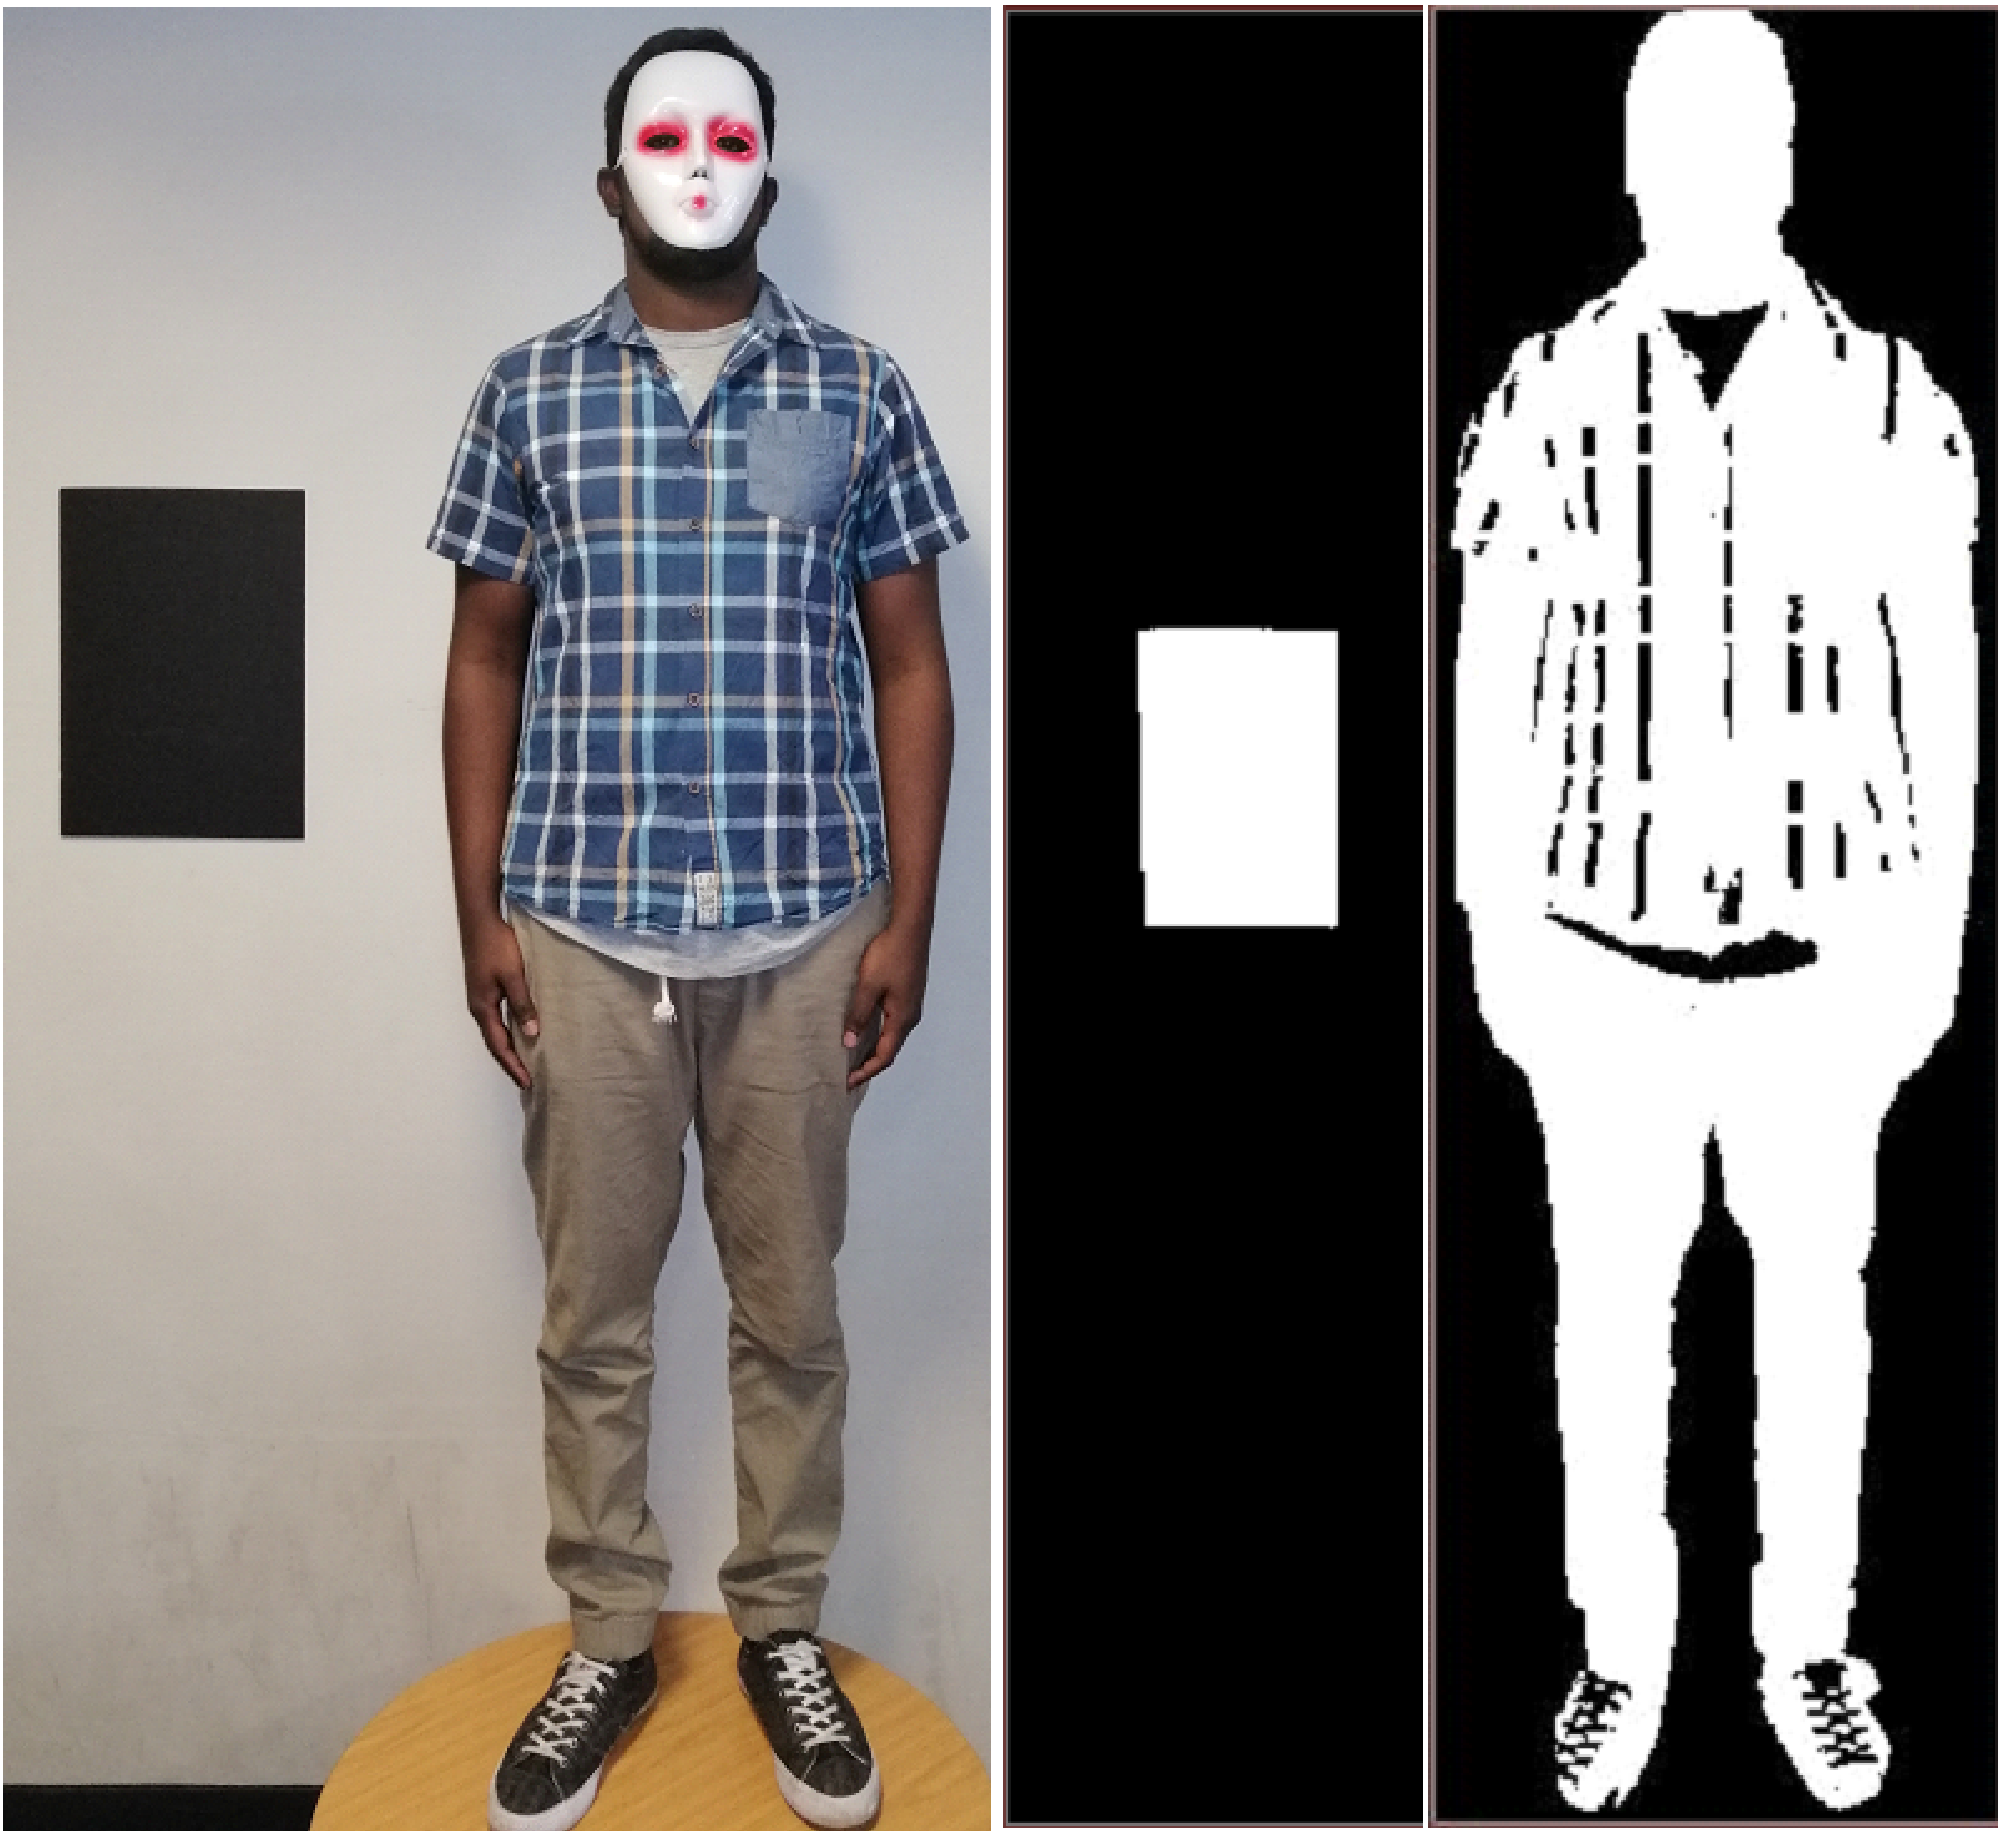
\includegraphics[width=0.5\linewidth]{segbeforeafter.png}
	\caption{Example photograph (left), reference object segmentation (middle), person segmentation (right).}
	\label{fig:segbeforeafter}
\end{figure}

\subsection{Machine Learning Layer}
\subsubsection{Model Choice and Evaluation}
As per consulting the aforementioned Literature Review, it was found that the simplest type of Neural Network that may account for a noisy, small, and potentially linearly inseparable data-set is the Multilayered Perceptron (MLP).
The Front, Side and Compensation models were all MLP's.
The models were evaluated by a weighted scoring system that took the maximum deviation from the mean as well as the Mean Absolute Error (MAE) into account.
MAE (measured in BMI) was considered as the main metric of model loss, since in this particular application, the accuracy of individual results was more important than evaluating the spread of BMI estimations \cite{bmifromface}.

\subsubsection{Training and Final Performance} \label{trainingandperformance}
The program filtered the dataset of features of points that contained errors from the Extraction Layer, leaving 427 points in the feature dataset.
Before training, 20\% of the feature dataset was removed to be used later as unseen data during model evaluation.
The remaining data was used with both the Classical Test-Train split and (Stratified) k-Fold cross validation methods to train the models.
The Classical method used a 70/30 train/test split for training, whilst the Cross Validation methods used 10 folds.

Different models were trained using different shuffles of data as well as different training parameters such as learning rate, batch size and number of epochs.
At the end of each complete training cycle, the models were evaluated by exposing them to the unseen data.
The model which had the lowest combination of MAE and maximum deviation when exposed to completely unseen data was saved as having the best performance.
The final Validation Model Loss and Training Method for the best performing models were as follows:
\begin{itemize}
\item Front: Trained using Stratified Cross Validation using 10 folds, Mean Absolute Error (MAE) — 3.32
\item Side: Trained using Cross Validation using 10 folds, MAE -- 2.77
\item Compensation: Trained using the Classical Test/Train Split, MAE -- 2.58
\end{itemize}
Note that the Front and Side View models were first trained, and the best performing models were used to generate data to train the Compensation model.
The full implementation of the system can be found at Ref \cite{repo}, and features a graphical user interface (GUI) for desktop computers.

\section{Sources of Error} \label{error}
As expected when performing feature extraction on a photographic dataset, the system design either had to account for or circumvent various errors in the dataset.
The following errors were circumvented by creating a Method One as described in Section \ref{refobdetseg}:
\begin{itemize}
	\item Poorly lit photographs, or non-uniform low-contrasting backgrounds that cause the RO to be confused with the background.
	\item The person being too close to or making contact with the RO.
	\item Another object being more to the left of the photograph than the RO.
\end{itemize}
The following errors were circumvented by combining the masks produced by foreground extraction and the Mask-RCNN:
\begin{itemize}
	\item The person being in contact with another object that would affect normal edge detection.
	\item The photograph containing other large objects that were in the foreground with the person.
\end{itemize}
Unfortunately there are some errors that could not be accounted for or circumvented, and must be prevented in any future data collection:
\begin{itemize}
	\item Taking front and side photographs from an angle such that the RO is seen as behind the person instead of alongside them, creating a distance perspective error.
	\item A more pronounced distance perspective error in all side photographs due to the RO being a person-width behind the side surface of the person being photographed.
	This results in the RO dimensions being slightly under-estimated, and the person's side dimensions being slightly exaggerated.
\end{itemize}

\section{Findings \& Analysis}
The models that were described has having the best performance to unseen data in Section \ref{trainingandperformance} was used to make BMI estimations for the entire dataset of 427 people.
Figures \ref{fig:spread} and \ref{fig:accuracies} show the BMI category composition of the dataset and average accuracy of the final BMI estimation (i.e. from the Compensator model), respectively, for each category.
Predictions on the total dataset had a mean absolute error of 3.2, and standard deviation of 3.9.
\begin{figure}
    \centering
    \begin{minipage}[b]{0.235\textwidth}
    	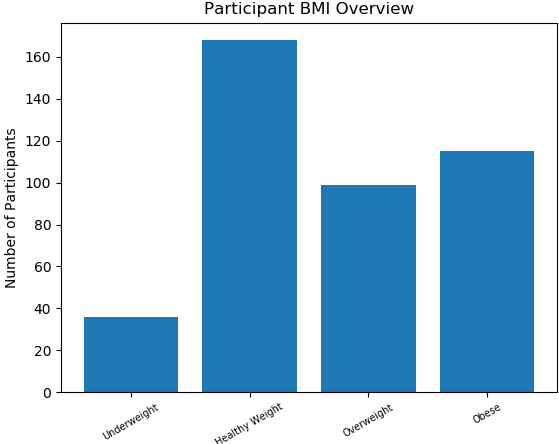
\includegraphics[width=\linewidth]{spread.png}
	\caption{Number of people in dataset according to BMI categories described in Section \ref{concept}).}
	\label{fig:spread}
    \end{minipage}
    \hspace{0.1cm}
    \begin{minipage}[b]{0.235\textwidth}
	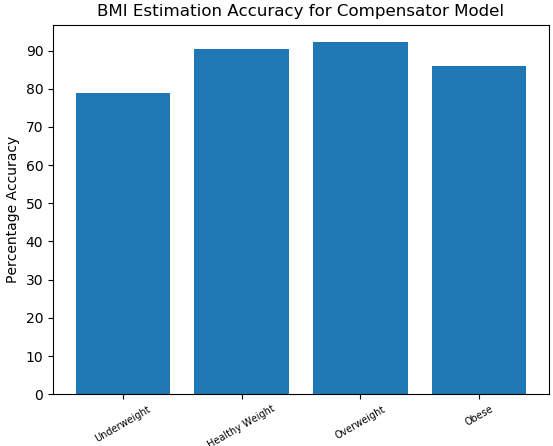
\includegraphics[width=\linewidth]{accuracies.png}
	\caption{Average accuracy of Final BMI Model estimations for total dataset according to BMI categories described in Section \ref{concept}).}
	\label{fig:accuracies}
    \end{minipage}
\end{figure}

The first thing to be noted from Figure \ref{fig:spread} is the sheer under-representation of the Underweight population in the dataset.
It thus comes as no surprise that the lowest BMI estimation accuracy comes from this group.
This is also seen in the low Front and Side model accuracies, as seen in Figures 6 - 17 in Appendix 5.
As seen, the performance of the Side model to Underweight participants had only 29\% of its category with an estimation error of less than 10\%.

Despite this, it appears that the results from the final compensation model show there is a definitive relationship between the maximum width and depth of the common areas body fat deposit and BMI, in reference to the well represented areas of the dataset, namely those of Healthy Weight and those Overweight.
This is seen in the mean estimation accuracy ranging between 79\% and 92\% throughout the BMI categories.
A more comprehensive view of the performance of the final model can be seen in the distribution of error of BMI estimations in Figure \ref{fig:errorspread}.

These figures show that approximately 61\% of all participants had an estimation error of 10\% or less -- the vast majority of which having measurement errors between 0 and 6\%.
With regards to the success criteria of a minimum mean accuracy of 75\%, these figures show that about 89\% of all participants had an estimation error of 25\% or less i.e. an estimation \textit{accuracy} of 75\% or more.
\begin{figure}
\centering
	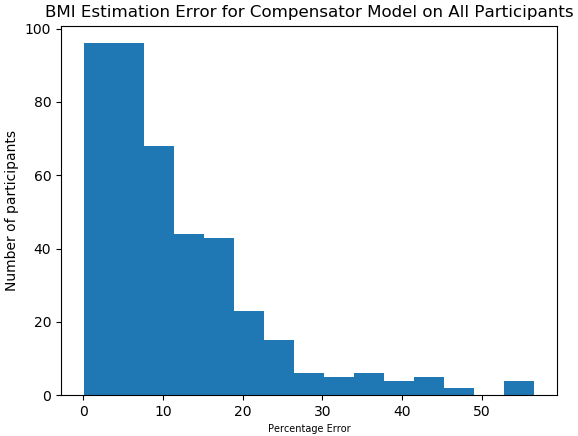
\includegraphics[width=0.65\linewidth]{errorspread.png}
	\caption{Frequency of Percentage Error for Final Model BMI Estimations performed on the Full Dataset.}
	\label{fig:errorspread}
\end{figure}

One notable misrepresentation shown by Figure \ref{fig:accuracies} however, is that there are approximately five people with a BMI over 45, seen in the data scatters in Appendix 5.
As expected, these outliers performed poorly in comparison to the categories where the majority of data was located, and has thus exaggerated the average error of the Obese category.
A better representation would be to evaluate the accuracies between an Obese BMI of 30 and 40, as they are better represented in the dataset, and extend the remaining points to differing levels of obesity.

Finally, we see that Figure 19 in Appendix 5 shows a slight 'flattening' or constant prediction across a small range of inputs.
This is most likely due to 'ReLu Neuron Death', which occurs when a ReLu-activated neuron receives an overall negative input, causing it to produce zero \cite{reludeath}.
It then follows that the constant output is produced since the constant bias term in a layer makes the majority (if not all) of the contribution to the output.
Alternatives that mitigate this are the Leaky/Parametric ReLu functions \cite{reludeath}, and should be considered in future to prevent this phenomenon.

\section{Additional Features}
The program allows for height and mass models to be trained, as to provide another means of BMI estimation.
The training and evaluation is the same as described above, producing the highest performing model.

The program also provides the user with the option to visualise the data being extracted from the image for the purpose of error detection.
This can be extended in future versions of the program to interactively choose a reference object in the photograph.

\section{Workflow and Project Management}
Appendix 1 contains the Division of Work, and Appendix 3 contains the original project schedule and allocated resources, all of which remained unchanged during the course of the project.
The project cost breakdown can be found in Appendix 5.
However it is worth noting that during the time allocated for Image Processing and Neural Network Testing, shown in Appendix 3, multiple extra tasks were completed, putting the group slightly ahead of schedule.
This included the Additional Features, unit testing on all non-library dependant elements of the software, and the design of the GUI for desktop use.

Using Git as source control, each group member worked on two separate trunks for each program layer.
Upon completing a task, the other group member reviewed the branch and approved merges into the master-branch when satisfied.
The use of GitKraken, which has a built-in own difference viewer, precluded the need to make use of pull requests on GitHub.

\section{Recommendations}
In accordance with Section \ref{error}, as to improve the quality of the training data as well as model performance, the following minor changes must be implemented when creating a dataset for this system in future:
\begin{itemize}
	\item There must be at least half a meter of space to the left of the RO in the photograph, as well as to the right of the person in the photograph.
	Having other objects vertically below the RO (especially of the same colour) or between the persons head and shoulder in the picture may interfere with detection.
	\item Consider making the RO a bright, distinctly coloured object worn on the person.
	This would improve the system's ability to locate the RO by first detecting the person, and using the same ROI to find the RO.
	This would also significantly reduce the distance perspective error discussed in Section \ref{error}.
\end{itemize}
With regards to the speed of execution and resource usage of the program, the following changes should also be implemented in future:
\begin{itemize}
	\item The program should be parallelised as far as possible.
	Processes such as RO detection and person detection are not required to be sequential.
	\item Instead of using the pre-trained Mask-RCNN model that is trained on 81 classes, train a new model on the same MS COCO dataset but only on two classes: person and background.
	This would decrease the size of the model, as well increase the speed of person detection.
\end{itemize}

\section{Conclusion}
The design and implementation of a software system that estimates BMI from a photograph has been presented.
This was accomplished by relating BMI to features including the estimated dimensions of common areas of body fat, silhouette area, and height.
These features were extracted using Computer Vision to perform Object Detection, Image Segmentation, Foreground Extraction and Size Estimation on front and side photographs of fully clothed people.
The features were then used to train three MLP models to perform BMI estimation.
The BMI estimation results of the final model showed a mean estimation accuracy ranging between 79\% and 92\% across BMI categories, fulfilling the minimum success criteria of 75\% mean accuracy.
Furthermore, the spread of error showed that 61\% of participants had an error less than 10\%, and 89\% of participants had an error less than 25\%.
Finally, this software has been presented with a GUI for medical practitioners to easily use.
It was noted that an increase in the size of the dataset as well as a revised placement and choice of reference object would result in more accurate feature extraction.
Hopefully in future, the additional features of height and mass estimation can be used alongside the BMI model to even more accurately determine these important metrics of health without patients needing to leave their home.

\section{Acknowledgements}
The author would like to extend his gratitude to the following people:
\begin{itemize}
    \item Sachin Govender (1036148) for his contribution, particularly to the Machine Learning layer of the system.
    His findings can be found in Ref \cite{sachin}.
    \item Prof. Scott Hazelhurst from the University of the Witwatersrand, who supervised this project.
    \item Dr. Neil Martinson from the Peri-Natal HIV Research Unit, who co-supervised this project.
    Dr. Martinson provided PHRU clinical research staff who were invaluable to this study due to their contribution to data collection.
\end{itemize}

\bibliographystyle{IEEEtran}
\bibliography{references}
\end{document}